% !TeX root = ./03_answers.tex

\documentclass[english]{scrartcl}
\usepackage[T1]{fontenc}
\usepackage[utf8]{inputenc}
\usepackage{multicol}
\usepackage{paralist}
\usepackage{hyperref}
\usepackage{listings}
\usepackage{fvextra} % loads also fancyvrb
\usepackage{pgfgantt}
\usepackage{amsmath}
\usepackage{xcolor}
\usepackage{dirtytalk}
\usepackage{xparse}
\usepackage{xpatch}
\usepackage[bottom=1.2in,top=1.2in]{geometry}
\usepackage{tikz}
\usetikzlibrary{arrows,automata,positioning}
\hypersetup{
    colorlinks,
    citecolor=black,
    filecolor=black,
    linkcolor=black,
    urlcolor=black
}
\lstset{
  basicstyle=\ttfamily,
  mathescape
}

\DeclareMathVersion{ttmath}
\DeclareSymbolFont{latinletters}{OT1}{\ttdefault}{m}{n}
%\SetSymbolFont{latinletters}{ttmath}{OT1}{\ttdefault}{m}{n}
\SetSymbolFont{letters}{ttmath}{OML}{ccm}{m}{it}
\SetSymbolFont{symbols}{ttmath}{OMS}{ccsy}{m}{n}
\SetSymbolFont{largesymbols}{ttmath}{OMX}{ccex}{m}{n}

% https://tex.stackexchange.com/questions/150965/insert-symbols-inside-verbatim-mode-latex/156419

\newcommand{\changeletters}{%
  \count255=`A
  \advance\count255 -1
  \loop\ifnum\count255<`Z
    \advance\count255 1
    \mathcode\count255=\numexpr\number\symlatinletters*256+\count255\relax
  \repeat
  \count255=`a
  \advance\count255 -1
  \loop\ifnum\count255<`z
    \advance\count255 1
    \mathcode\count255=\numexpr\number\symlatinletters*256+\count255\relax
  \repeat
  \count255=`0
  \advance\count255 -1
  \loop\ifnum\count255<`9
    \advance\count255 1
    \mathcode\count255=\numexpr\number\symlatinletters*256+\count255\relax
  \repeat
}

\xapptocmd{\ttfamily}{\mathversion{ttmath}\changeletters}{}{}

\setkomafont{disposition}{\normalfont\bfseries}
\definecolor{light-gray}{gray}{0.95}

\begin{document}

\NewDocumentCommand{\codeword}{v}{%
\colorbox{light-gray}{\texttt{\textcolor{black}{#1}}}%
}

% == START: TITLE == %

\subtitle{6CCS3CFL - Compilers \& Formal Languages}
\title{Homework 3}
\author{Finley Warman}
\date{\today}

\maketitle

% == END: TITLE == %
% == START: CONTENTS == %

\tableofcontents
\par\noindent\rule{\textwidth}{0.4pt}

% == END: CONTENTS == %

\newpage

% MAIN CONTENT:

\addcontentsline{toc}{section}{Question 1}
\section*{Question 1}
Q: The regular expression matchers in Java, Python and Ruby can be very slow with some (basic) regular expressions. What is the main reason for this inefficient computation?
\\
\\
A: These languages construct an equivalent NFA to the input regular expression `under the hood'.
Translating these expressions into NFAs can cause the size of the resulting automaton to grow (typically O(n) space).
Testing to see if the automaton accepts the input string is done often with a depth-first search, which can be slow for these large inputs as
backtracking is required if visiting a `wrong' path to an accepting state.

\addcontentsline{toc}{section}{Question 2}
\section*{Question 2}
Q: What is a regular language? Are there alternative ways to define this notion? If yes, give an explanation why they define the same notion
\\
\\
A: A regular language is a language that can be expressed by a regular expression. This is equivalent to a language that can be described with a finite automaton (NFA or DFA).
These notions are the same, since all NFAs can be converted to equivalent DFAs, and we know from Thompson that a regular expression can be converted to a NFA.

\addcontentsline{toc}{section}{Question 3}
\section*{Question 3}
Q: Why is every finite set of strings a regular language?
\\
\\
A: A high-level explanation: for any finite set of strings, we can simply construct an NFA with one 'branch' leading to a linear DFA for each string in the language. \\
We can also say that since all single strings are regular, and any union of two regular languages is regular, then this finite set of strings can be constructed from the union of the languages containing each string, and is therefore regular.


\addcontentsline{toc}{section}{Question 4}
\section*{Question 4}
Q: Assume you have an alphabet consisting of the letters a, b and c only. \\
(1) Find a regular expression that recognises the two strings ab and ac. \\
(2) Find a regular expression that matches all strings except these two strings.
\\
\\
A: 1) \verb~ (a.(b+c)) ~ \\
A: 2) \verb~ a* + (a.a*.(b+c).(a+b+c)*) + ((b+c).(a+b+c)*)~ \\
\newpage
NFA for this expression:

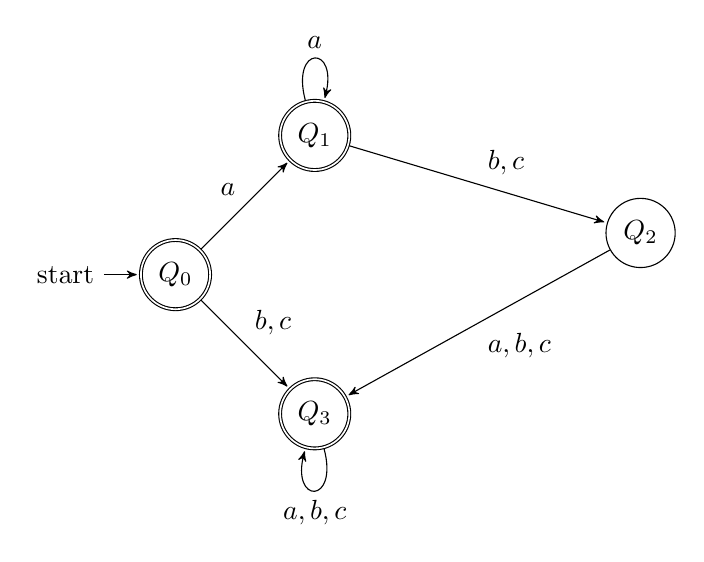
\begin{tikzpicture}[->,>=stealth',shorten >=1pt,auto,node distance=2.5cm,
    scale = 1,transform shape]

\node[state,accepting,initial] (Q_0) {$Q_0$};
\node[state,accepting] (Q_1) [above right of=Q_0] {$Q_1$};
\node[state] (Q_2) [below right=0.6cm and 3.5cm of Q_1] {$Q_2$};
\node[state,accepting] (Q_3) [below right of=Q_0] {$Q_3$};

\path
    (Q_0) edge              node {$a$} (Q_1)
    (Q_1) edge [loop above] node {$a$} (Q_1)
    (Q_1) edge              node {$b,c$} (Q_2)
    (Q_2) edge              node {$a,b,c$} (Q_3)
    (Q_0) edge              node {$b,c$} (Q_3)
    (Q_3) edge [loop below] node {$a,b,c$} (Q_3);

\end{tikzpicture}

\addcontentsline{toc}{section}{Question 5}
\section*{Question 5}
Q: Given the alphabet \{a,b\}.
Draw the automaton that has two states, say $Q_0$ and $Q_1$.  \\
The starting state is $Q_0$ and the final state is $Q_1$. \\
The transition function is given by:
\begin{verbatim}
    (Q0,a)→Q0
    (Q0,b)→Q1
    (Q1,b)→Q1
\end{verbatim}

A: Finite State Machine:

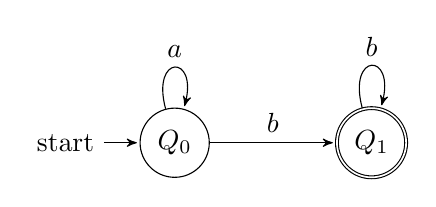
\begin{tikzpicture}[->,>=stealth',shorten >=1pt,auto,node distance=2.5cm,
    scale = 1,transform shape]

\node[state,initial] (Q_0) {$Q_0$};
\node[state,accepting] (Q_1) [right of=Q_0] {$Q_1$};

\path
    (Q_0) edge [loop above] node {$a$} (Q_0)
    (Q_0) edge              node {$b$} (Q_1)
    (Q_1) edge [loop above] node {$b$} (Q_1);

\end{tikzpicture}

What does this language accept? \\
Any number of `a' followed by 1 or more `b'. (\verb~a*b+~)

\addcontentsline{toc}{section}{Question 6}
\section*{Question 6}
Q: Give a non‑deterministic finite automaton that can recognise the language \verb~L(a·(a+b)*·c)~ \\

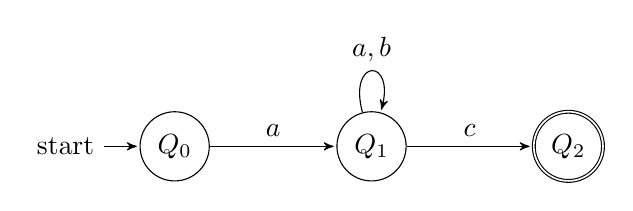
\begin{tikzpicture}[->,>=stealth',shorten >=1pt,auto,node distance=2.5cm,
    scale = 1,transform shape]

\node[state,initial] (Q_0) {$Q_0$};
\node[state] (Q_1) [right of=Q_0] {$Q_1$};
\node[state,accepting] (Q_2) [right of=Q_1] {$Q_2$};

\path
    (Q_0) edge              node {$a$} (Q_1)
    (Q_1) edge [loop above] node {$a,b$} (Q_1)
    (Q_1) edge              node {$c$} (Q_2);

\end{tikzpicture}

\newpage

\addcontentsline{toc}{section}{Question 7}
\section*{Question 7}
Given a DFA $A(\Sigma , Q, Q_0, F, \delta)$, the language accepted by this DFA, $L$, is described as
$L = \{ s \; | \; \hat{\delta}( Q_0 , s ) \in F \}$ - that is, all strings $s$ which the automaton accepts (there is a set of transitions for each consecutive character in the string to some accepting state).
\\
\\
For an NFA $A(\Sigma , Q_s, Q_{0s}, F, \rho)$, the language $L$ is $L = \{ s \; | \; \hat{\rho}( Q_{0s} , s ) \in F \}$. (All strings accepted by the NFA)

\addcontentsline{toc}{section}{Question 8}
\section*{Question 8}
Q: Find an automaton recognising complement language, over alphabet \{a, b\}\\
\\
A:
To convert an automaton to its complement, first 'complete' it (e.g. by adding a 'sink state' for all missing transitions), then swap all accepting and non-accepting states:

% ORIGINAL
% \begin{tikzpicture}[->,>=stealth',shorten >=1pt,auto,node distance=2.5cm,
%   scale = 1,transform shape]

% \node[state, initial] (Q_0) {$Q_0$};
% \node[state, accepting] (Q_1) [right of=Q_0] {$Q_1$};

% \path
%   (Q_0) edge              node {$a$} (Q_1)
%   (Q_1) edge [loop above] node {$b$} (Q_1)
% ;
% \end{tikzpicture}

% COMPLEMENT
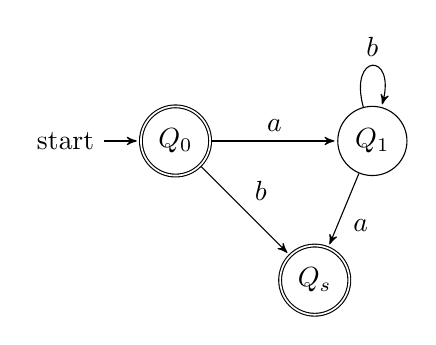
\begin{tikzpicture}[->,>=stealth',shorten >=1pt,auto,node distance=2.5cm,
  scale = 1,transform shape]

\node[state, initial, accepting] (Q_0) {$Q_0$};
\node[state] (Q_1) [right of=Q_0] {$Q_1$};
\node[state, accepting] (Q_s) [below right of=Q_0] {$Q_s$};

\path
  (Q_0) edge              node {$a$} (Q_1)
  (Q_0) edge              node {$b$} (Q_s)

  (Q_1) edge              node {$a$} (Q_s)
  (Q_1) edge [loop above] node {$b$} (Q_1)
;
\end{tikzpicture}

\addcontentsline{toc}{section}{Question 9}
\section*{Question 9}

Q: Convert NFA over \{a,b\} to DFA:\\
\\
A:

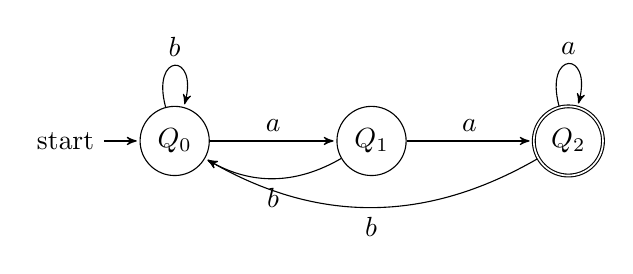
\begin{tikzpicture}[->,>=stealth',shorten >=1pt,auto,node distance=2.5cm,
  scale = 1,transform shape]

\node[state, initial] (Q_0) {$Q_0$};
\node[state] (Q_1) [right of=Q_0] {$Q_1$};
\node[state, accepting] (Q_2) [right of=Q_1] {$Q_2$};

\path
  (Q_0) edge              node {$a$} (Q_1)
  (Q_0) edge [loop above] node {$b$} (Q_0)

  (Q_1) edge              node {$a$} (Q_2)
  (Q_1) edge [bend left]  node {$b$} (Q_0)

  (Q_2) edge [loop above] node {$a$} (Q_2)
  (Q_2) edge [bend left]  node {$b$} (Q_0)
;
\end{tikzpicture}

\addcontentsline{toc}{section}{Question 10}
\section*{Question 10}

Q: Find corresponding minimal automaton for DFA over \{0,1\}. \\
\\
A:


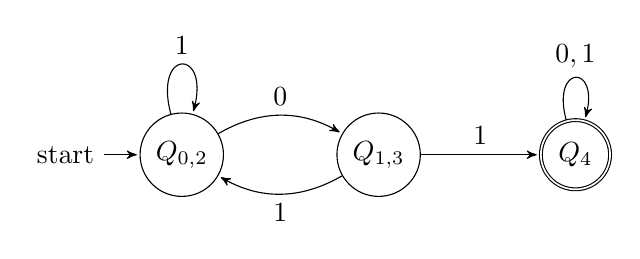
\begin{tikzpicture}[->,>=stealth',shorten >=1pt,auto,node distance=2.5cm,
  scale = 1,transform shape]

\node[state, initial] (Q_0) {$Q_{0,2}$};
\node[state] (Q_1) [right of=Q_0] {$Q_{1,3}$};
\node[state, accepting] (Q_4) [right of=Q_1] {$Q_4$};

\path
  (Q_0) edge [loop above]  node {$1$} (Q_0)

  (Q_0) edge [bend left]   node {$0$} (Q_1)
  (Q_1) edge [bend left]   node {$1$} (Q_0)

  (Q_1) edge               node {$1$} (Q_4)

  (Q_4) edge [loop above]  node {$0,1$} (Q_4)


;
\end{tikzpicture}

\addcontentsline{toc}{section}{Question 11}
\section*{Question 11}

Q: Give a regular expression recognising the same language as DFA over \{a,b\}. \\
\\
A: \verb~ (b+ab+aa(a*)b)*aa(a)* ~

\addcontentsline{toc}{section}{Question 12}
\section*{Question 12}
Q: How many (maximum) states does a DFA need to match an equivalent DFA with $n$ states?\\
A: $2^n$

\addcontentsline{toc}{section}{Question 13}
\section*{Question 13}
Q: Prove for all regular expressions $r$ we have $nullable(r)$ iff $[] \in L(r)$
\\
$nullable$ definition:
\begin{verbatim}
  nullable(r): match r => Boolean
    case 0        == false
    case 1        == true
    case c        == false
    case r1+r2    == nullable(r1) || nullable(r2)
    case r1.r2    == nullable(r1) && nullable(r2)
    case r*       == true
\end{verbatim}
\mbox{ }\\

For expressions of the forms \textbf{0} and c, nullable(r) does not hold, and $[] \notin L(r)$. \\

For expressions of the form \textbf{1}, $[] \in L(r)$ holds by definition. \\

In the case of $r^*$, $[] \in L(r)$ since $r^*$ matches 0-or-more of r, which includes the empty string. \\

The final two cases are defined recursively in terms of nullable(r), and possible cases are covered as above. \\

For an expression $r$ of the form $r_1 + r_2$, then either $r_1$ or $r_2$ must be nullable for $nullable(r)$ to hold.
For an expression $r$ of the form $r_1 . r_2$, then both $r_1$ and $r_2$ must be nullable for $nullable(r)$ to hold.

As from the above defintions, we know that if nullable(r) holds for these two cases, then $[] \in L(r)$, otherwise, $[] \notin L(r)$.

\end{document}
